\section{Introdução}

O presente trabalho tem como objetivo estudar o controle de um sistema de levitação magnética por meio de um controlador PID em malha fechada. O sistema analisado é composto por uma peça submetida à ação da gravidade e a uma força magnética dependente da corrente elétrica e da posição da peça em relação ao atuador. A proposta central consiste em determinar condições nas quais o sistema pode ser estabilizado em torno de uma posição de equilíbrio, mesmo na presença de pequenas perturbações.

Para a modelagem, começamos utilizando as equações diferenciais que descrevem a dinâmica elétrica e mecânica do   levitador, adotando como ponto de operação uma condição de equilíbrio em que a força magnética compensa exatamente o peso da peça. A partir desse ponto, é introduzido um controlador PID, cuja função é ajustar a tensão aplicada ao circuito para corrigir desvios na posição em relação ao valor desejado.

Além da análise do caso ideal, sem incertezas de medição, estaremos investigando a influência de  ruído aditivo na malha de realimentação. 

Dessa forma, busca-se avaliar não apenas a capacidade do controlador em estabilizar o sistema, mas também sua sensibilidade a perturbações e imperfeições no processo de medição. Os resultados são obtidos por meio de simulações numéricas do modelo em espaço de estados, permitindo analisar a resposta temporal do sistema e os limites de estabilidade para diferentes condições.

\section{Projeto do controlador PID}

Para estabilizar a posição da peça em torno do ponto de equilíbrio $x_0$, foi adotado um controlador PID. Como o sistema em malha aberta é naturalmente instável nas proximidades desse ponto, o controlador atua corrigindo a tensão aplicada à bobina sempre que há desvio entre a posição atual e a posição de referência.

A variável de erro foi definida como a diferença entre a posição instantânea e a posição desejada,
isto é,
  \[
  e(t) = x(t) - x_0.
  \]

A tensão aplicada ao sistema foi escrita como a soma entre a tensão de equilíbrio $u_0$ e uma parcela corretiva $\Delta u(t)$, fornecida pelo controlador. Assim, a lei de controle adotada foi

  \[
  u(t) = u_0 + \Delta u(t),
  \]
  com
  \[
  \Delta u(t) = K_p e(t) + K_i E(t) + K_d \dot{e}(t),
  \]
  sendo
  \[
  \dot{E}(t) = e(t).
  \]

Nessa formulação, o termo proporcional reage imediatamente ao erro de posição, aumentando a ação de controle quando a peça se afasta do ponto de referência. O termo integral acumula o erro ao longo do tempo e contribui para reduzir desvios persistentes em regime permanente. Já o termo derivativo atua com base na taxa de variação do erro, introduzindo amortecimento na resposta e ajudando a reduzir oscilações.

No modelo implementado, o controlador PID foi incorporado diretamente à representação em espaço de estados por meio da inclusão da variável $E(t)$, associada à integral do erro. Dessa forma, o vetor de estados passou a ser composto por corrente, posição velocidade e estado integral, permitindo simular de forma conjunta a dinâmica da planta e a dinâmica do controlador.

A sintonia dos ganhos foi realizada de forma numérica e iterativa, buscando-se um conjunto de  parâmetros capaz de estabilizar o sistema para pequenas perturbações na posição inicial, conforme solicitado no enunciado. No conjunto final utilizado no notebook, foram adotados os ganhos

  \[
  K_p = 8000, \qquad K_i = 4000, \qquad K_d = 150.
  \]

Esses valores produziram uma resposta estável para perturbações pequenas, com retorno da posição à
vizinhança do ponto de equilíbrio e corrente limitada ao intervalo admissível do sistema.

De forma qualitativa, o ganho proporcional foi responsável por tornar a correção suficientemente forte para reagir ao deslocamento da peça, o ganho integral melhorou a eliminação do erro residual, e o ganho derivativo contribuiu para reduzir oscilações e suavizar a convergência. Como se trata de um sistema não linear e sensível à posição, a escolha desses ganhos envolveu compromisso entre rapidez de resposta, limitação da corrente e manutenção da estabilidade.

\section{ Resultados da Atividade 1: resposta temporal e faixa estável de $\epsilon$.}

Na primeira etapa, analisou-se o comportamento do sistema em malha fechada para uma pequena perturbação na posição inicial, conforme proposto no enunciado. Para isso, foi considerada a condição inicial
  \[
  x(0) = x_0 + \epsilon,
  \]
  com
  \[
  \epsilon = 0{,}02x_0,
  \]

o que corresponde a uma perturbação de $2\%$ em relação à posição de
equilíbrio.

Os resultados obtidos indicam que o controlador PID foi capaz de estabilizar o sistema para essa condição inicial. A evidência principal disso está na resposta temporal da posição e da velocidade da peça. Observa-se que a posição retorna à vizinhança de $x_0$ ao longo do tempo, enquanto a velocidade tende a zero, caracterizando a convergência do sistema para um estado estável.

  \begin{figure}[H]
      \centering
       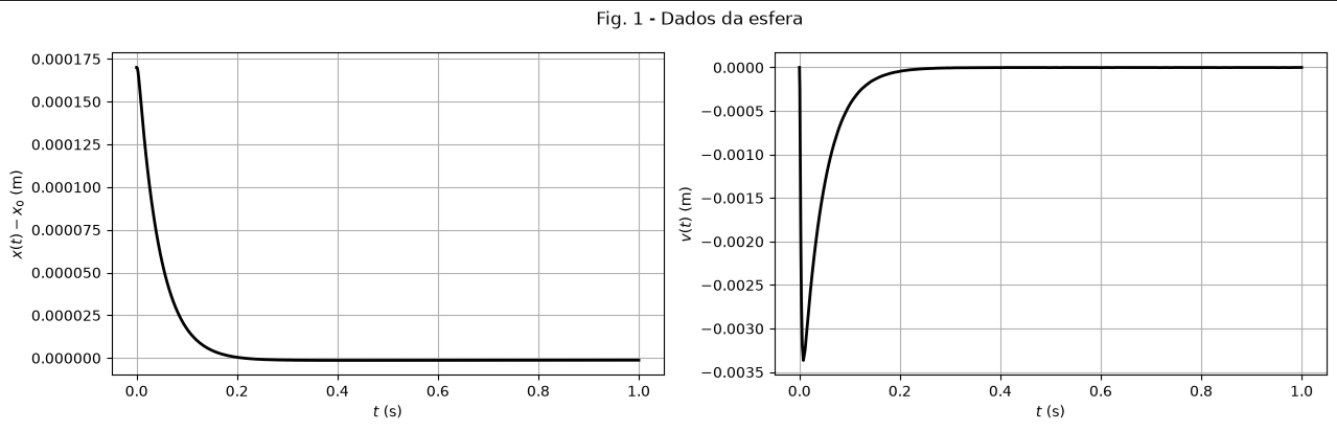
\includegraphics[width=0.9\textwidth]{imagens/grafico_posicao_velocidade.png}
      \caption{Resposta temporal da posição e da velocidade da peça para uma
      perturbação inicial de $2\%$ em relação a $x_0$.}
      \label{fig:posicao_velocidade_atividade1}
  \end{figure}

A Figura~\ref{fig:posicao_velocidade_atividade1} mostra que, após o deslocamento inicial, a peça não se afasta indefinidamente da posição de referência nem apresenta crescimento oscilatório. Pelo contrário, a trajetória permanece limitada e evolui em direção ao ponto de equilíbrio. Esse comportamento confirma que a ação de controle foi suficiente para compensar o efeito da perturbação inicial.

Do ponto de vista físico, isso significa que o controlador ajusta a tensão aplicada à bobina de modo a modificar a corrente elétrica e, consequentemente, a força magnética atuante sobre a peça. Esse mecanismo permite corrigir o desvio de posição e restabelecer o equilíbrio dinâmico do sistema.

Além da posição e da velocidade, a corrente elétrica também constitui uma evidência importante da atuação do controlador, pois representa diretamente o esforço de controle necessário para estabilizar o sistema. A análise desse sinal permite verificar se a correção exigida da fonte permanece dentro do limite admissível de operação.

  % Inserir aqui o gráfico da corrente
  \begin{figure}[H]
      \centering
       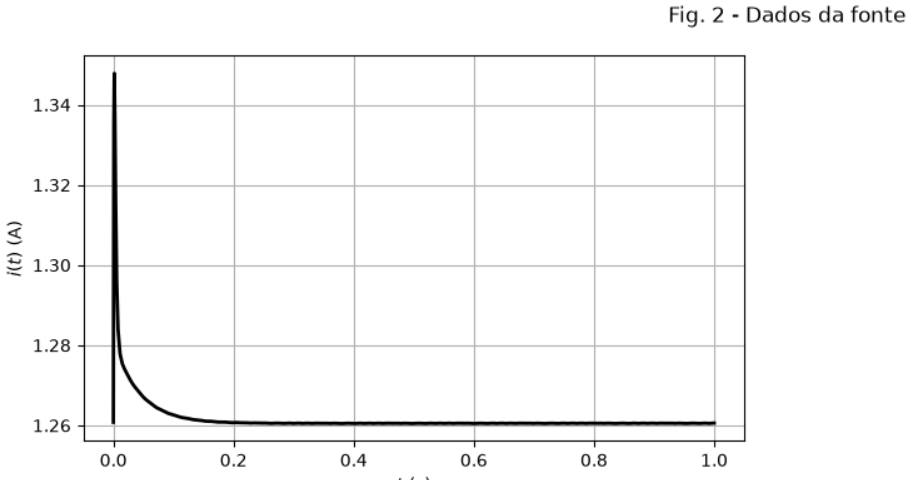
\includegraphics[width=0.75\textwidth]{imagens/grafico_corrente.png}
      \caption{Evolução temporal da corrente elétrica durante a estabilização do
      sistema para $\epsilon = 2\%$.}
      \label{fig:corrente_atividade1}
  \end{figure}

Os gráficos apresentados nas Figuras~\ref{fig:posicao_velocidade_atividade1} e~\ref{fig:corrente_atividade1} mostram que o controlador PID foi capaz de estabilizar o sistema para uma perturbação inicial de $2\%$. Observa-se que a posição retorna à vizinhança de $x_0$, enquanto a velocidade tende a zero ao longo do tempo, sem indicação de comportamento divergente. Além disso, a corrente permanece dentro do limite máximo de $2\,\text{A}$, mostrando que a estabilização ocorre de forma compatível com a restrição imposta à fonte.

Entretanto, esse resultado ainda corresponde a um caso particular. Para avaliar a faixa de perturbações iniciais para as quais o sistema permanece estável, foi realizada uma varredura numérica dos valores de $\epsilon$, sempre verificando também a restrição de corrente máxima. A partir dessa análise, obteve-se
\[
\epsilon_{\max} \approx 0{,}001165\ \text{m},
\]
o que corresponde a aproximadamente $13{,}71\%$ da posição de equilíbrio $x_0$.

\section{Resultados da Atividade 2: efeito do ruído na malha de realimentação}

  Na Atividade 2, foi introduzido ruído na medição da posição da peça, com média
  zero e desvio padrão dado por
  \[
  sd = 0{,}04x_0.
  \]

Com isso, o controlador PID passa a atuar sobre sinais medidos com incerteza, o que torna a malha mais sensível e dificulta a estabilização do sistema, principalmente devido ao termo derivativo.

  \begin{figure}[H]
      \centering
       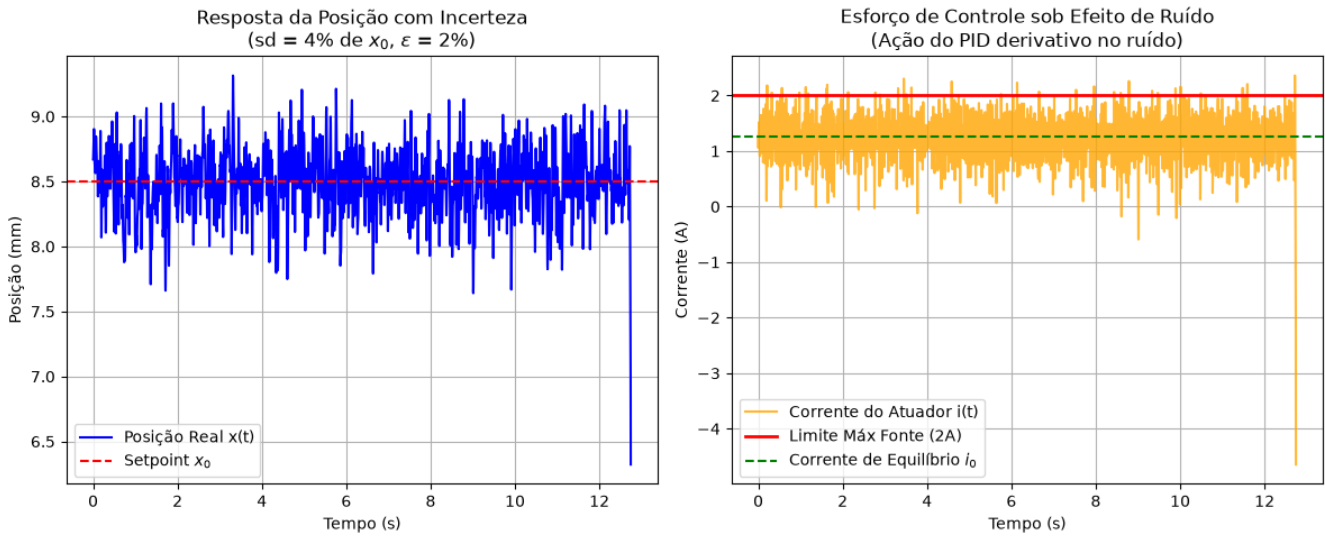
\includegraphics[width=0.9\textwidth]{imagens/grafico_ruido.png}
      \caption{Resposta do sistema com ruído na malha de realimentação.}
      \label{fig:ruido_atividade2}
  \end{figure}

A Figura~\ref{fig:ruido_atividade2} mostra que a presença de ruído prejudica o desempenho do controlador em comparação com o caso ideal. Além disso, a faixa de valores de $\epsilon$ para a qual o sistema permanece estável é reduzida, e o aumento de $sd$ torna a estabilidade ainda mais difícil de manter.

Assim, os resultados indicam que o controlador foi eficaz no caso ideal, mas se mostrou sensível à incerteza na medição.

\section{Conclusão}

Neste trabalho, foi possível modelar o sistema de levitação magnética em espaço de estados e aplicar um controlador PID para estabilizar a posição da peça em torno do ponto de equilíbrio. Na Atividade 1, os resultados mostraram que o controlador foi capaz de estabilizar o sistema para pequenas perturbações iniciais, mantendo também a corrente dentro do limite especificado.

Na Atividade 2, observou-se que a presença de ruído na malha de realimentação prejudica o desempenho do controlador e reduz a faixa de estabilidade do sistema. Assim, conclui-se que o PID adotado foi eficaz no caso ideal, mas apresenta sensibilidade à incerteza de medição.